\par
\chapter{Repositorios y evidencia complementaria}

Los recursos técnicos proporcionados se encuentran en los siguientes repositorios:

Contenedores Docker:

\href{https://github.com/YahayUniversidad/IADegreeThesis/tree/main/Contenedores}{https://github.com/YahayUniversidad/IADegreeThesis/tree/main/Contenedores}\\

Desarrollo de la solución: 

\href{https://github.com/YahayUniversidad/IADegreeThesis/tree/main/Desarrollo}{https://github.com/YahayUniversidad/IADegreeThesis/tree/main/Desarrollo}\\

Documentación relacionada:

\href{https://github.com/YahayUniversidad/IADegreeThesis/tree/main/DocumentosBase}{https://github.com/YahayUniversidad/IADegreeThesis/tree/main/DocumentosBase}\\

Para una reproducción verificable, la versión final debe asociar los enlaces con un commit o etiqueta estable e indicar qué script genera cada tabla, figura y modelo.

\section{Capturas adicionales de dashboards}

\begin{figure}[h!]
    \centering
    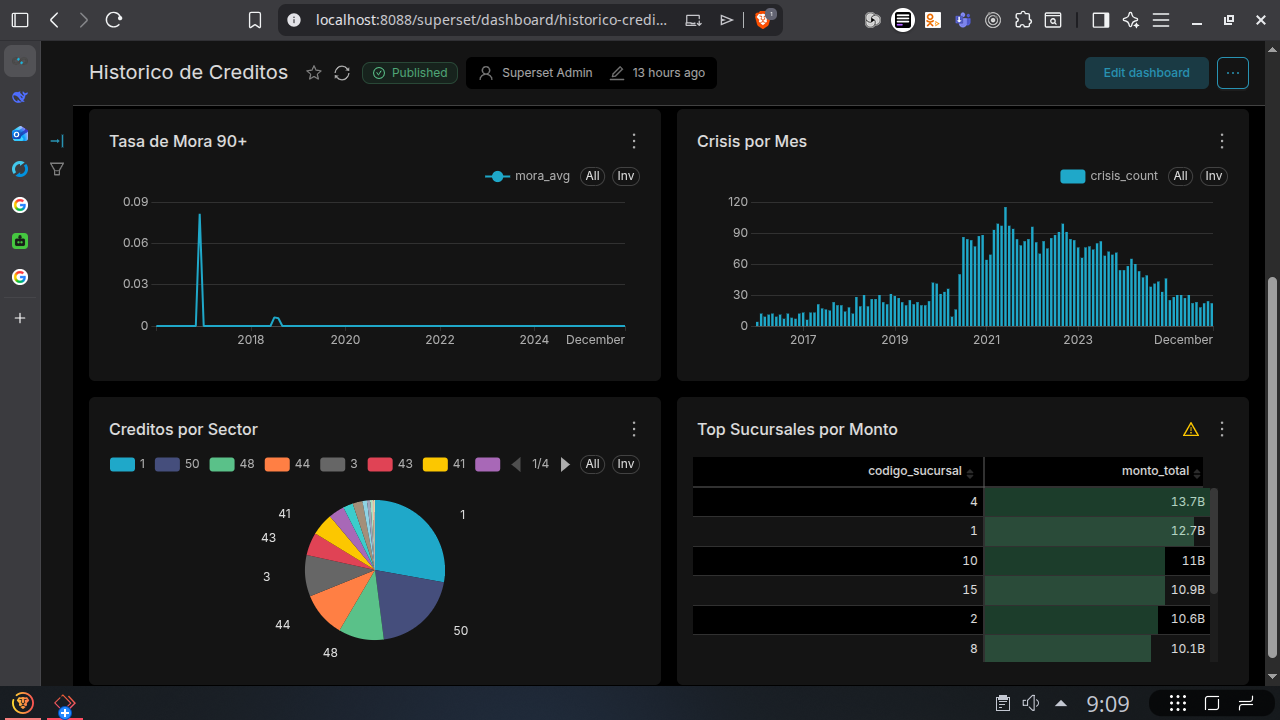
\includegraphics[width=0.8\textwidth]{images/dw-01-historicoCreditos2.png}
    \caption{Vista complementaria del dashboard histórico de créditos.}
    \label{fig:appendix_historico}
\end{figure}

\begin{figure}[h!]
    \centering
    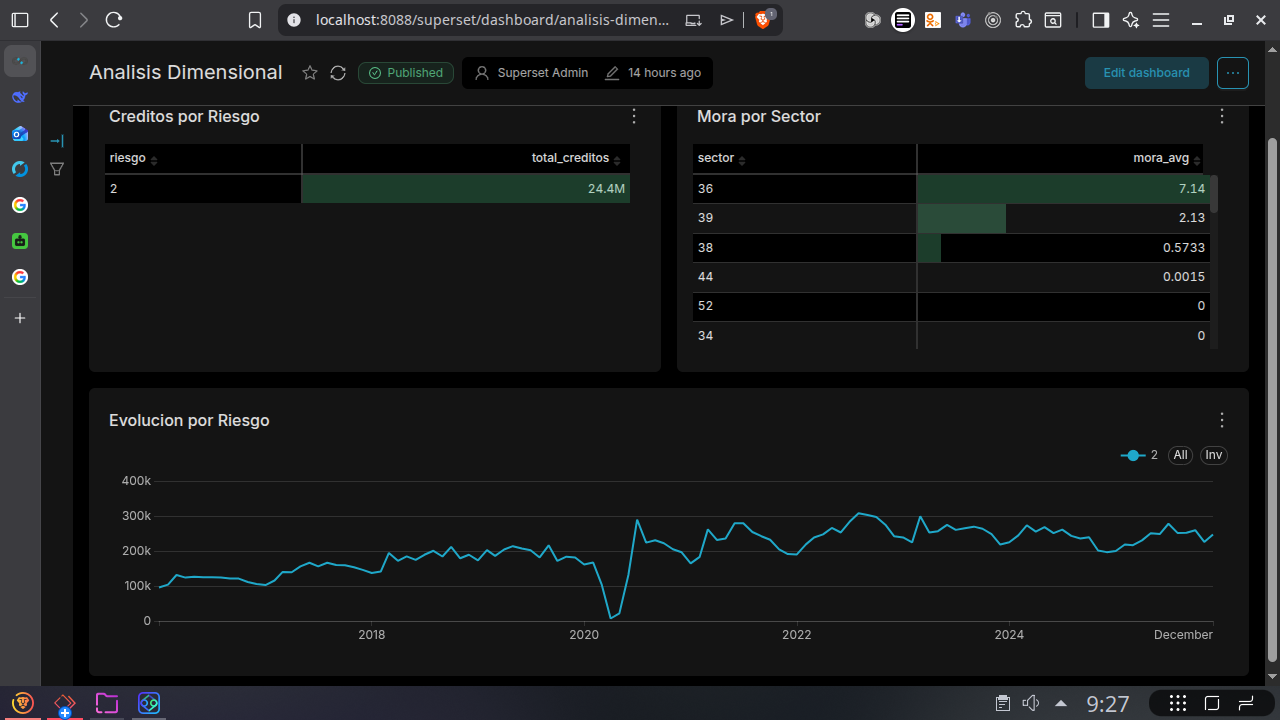
\includegraphics[width=0.8\textwidth]{images/dw-02-AnalisisDimensional.png}
    \caption{Dashboard de análisis dimensional por riesgo y sector.}
    \label{fig:appendix_dimensional}
\end{figure}

\begin{figure}[h!]
    \centering
    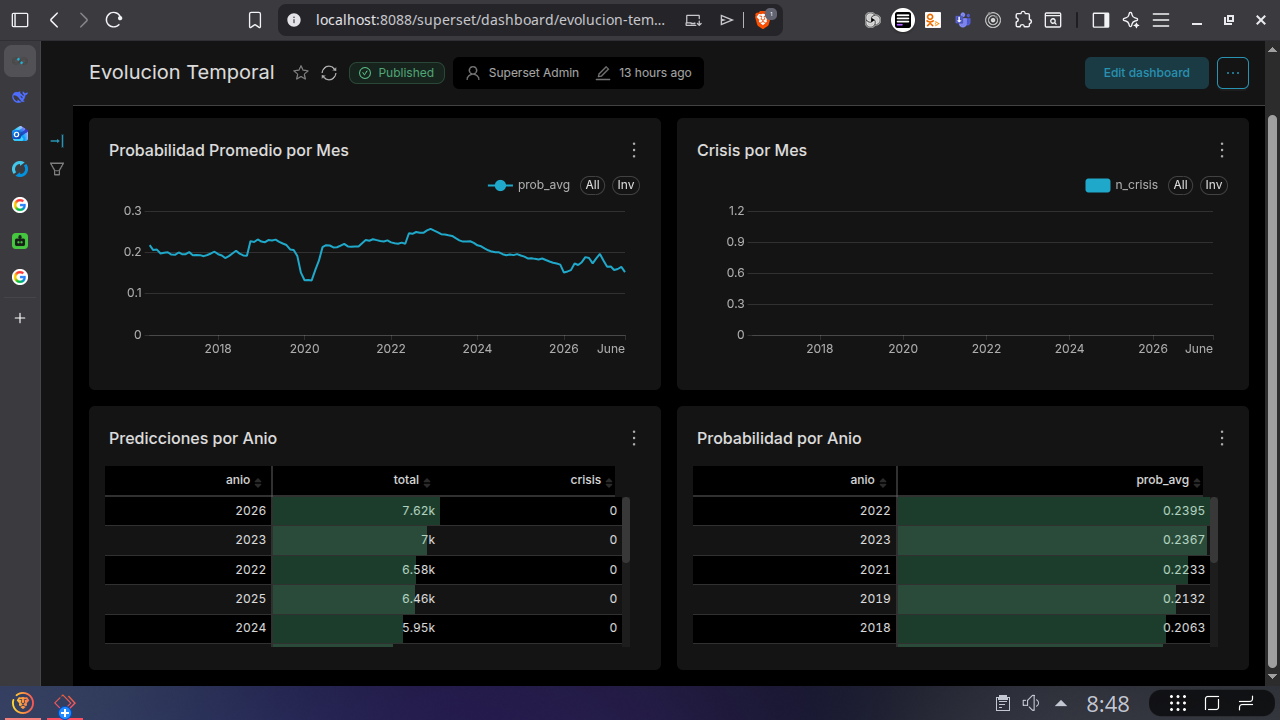
\includegraphics[width=0.8\textwidth]{images/dw-06-evolucionTemporal.png}
    \caption{Dashboard de evolución temporal de predicciones.}
    \label{fig:appendix_evolucion}
\end{figure}

\section{Información mínima para reproducibilidad}

La documentación final del repositorio debería incluir: definición de las ocho reglas de \texttt{crisis\_flag}; diccionario de las veintiuna características; conteos de registros y secuencias por etapa; particiones temporales; configuración completa de CNN, MLP y LightGBM; semillas; versiones de librerías; especificaciones de hardware; hashes o versiones de datos; métricas por horizonte; y procedimientos para ejecutar los DAG y reconstruir los dashboards.

\section{Esquema estrella del datamart}

El datamart analítico utiliza un esquema estrella con dos tablas de hechos que comparten las mismas dimensiones. A continuación se presentan los diagramas de cada tabla de hechos.

\subsection{Tabla de hechos: fact\_creditos\_mensual}

\begin{figure}[h!]
    \centering
    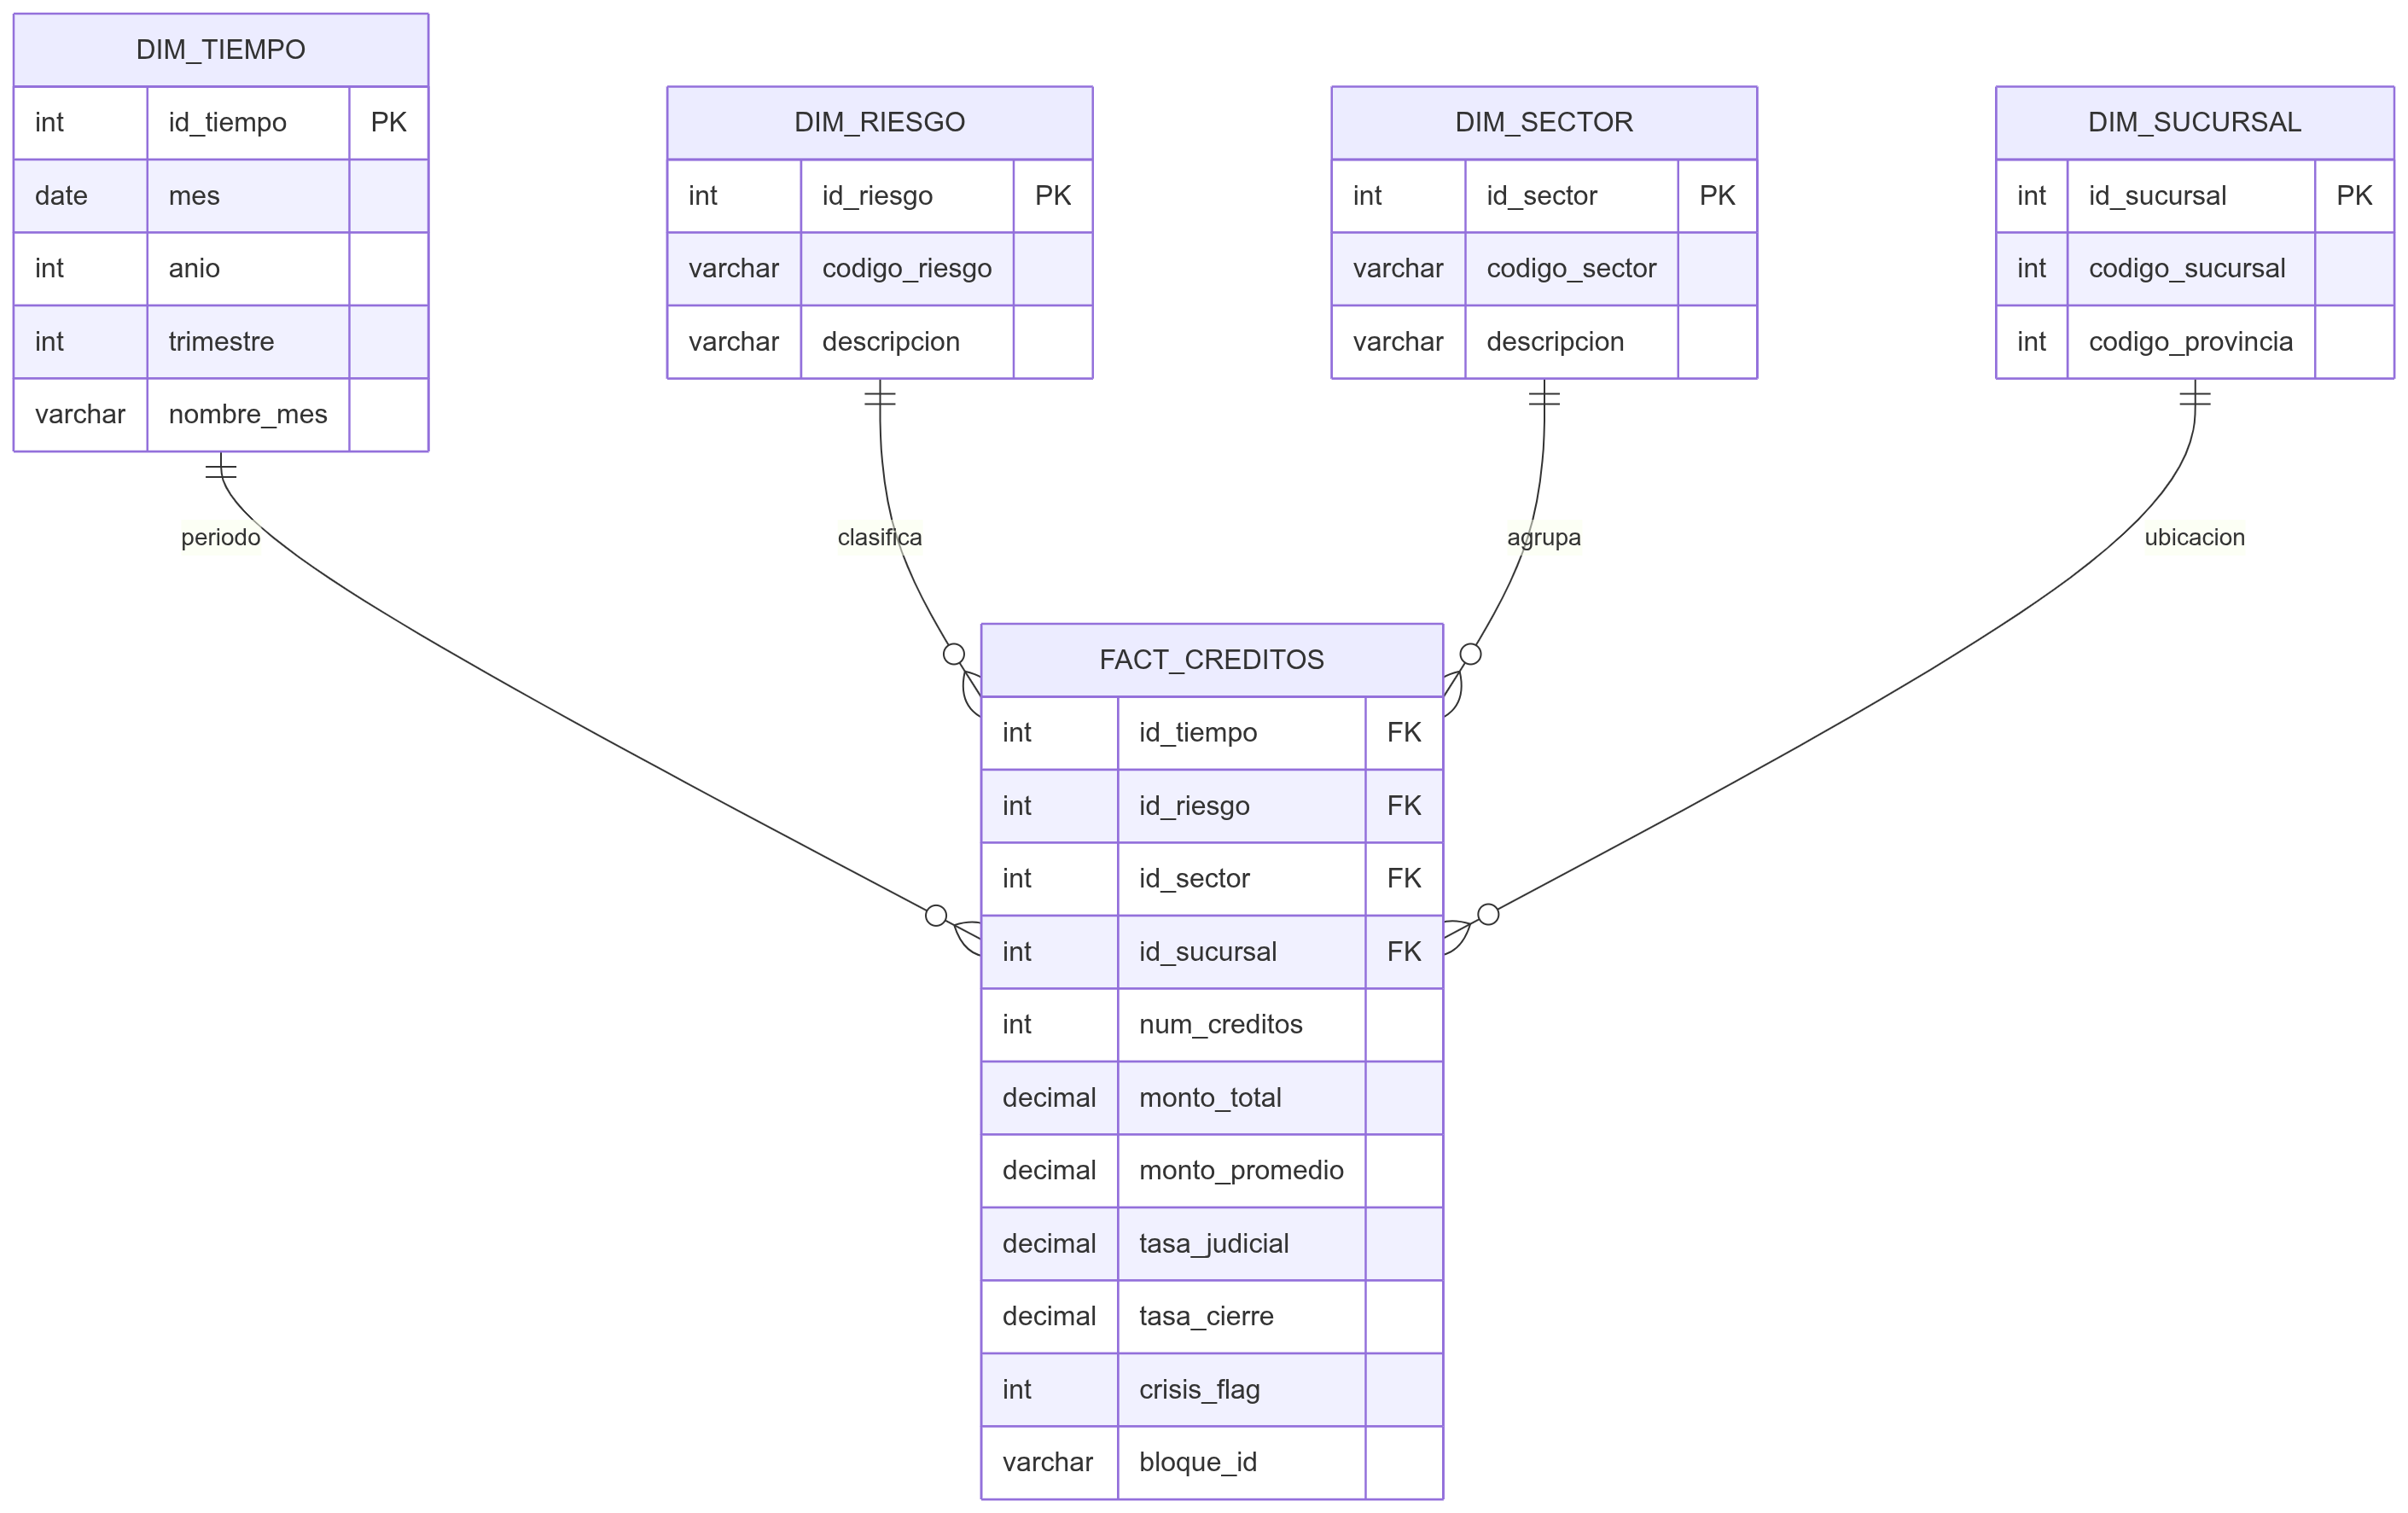
\includegraphics[width=1.0\textwidth]{images/MM-08a Estrella para fact_creditos_mensual.png}
    \caption{Esquema estrella de la tabla \texttt{fact\_creditos\_mensual}. Almacena los agregados históricos de créditos por bloque-mes, incluyendo la variable objetivo \texttt{crisis\_flag}.}
    \label{fig:appendix_estrella_creditos}
\end{figure}

\subsection{Tabla de hechos: fact\_predicciones}

\begin{figure}[h!]
    \centering
    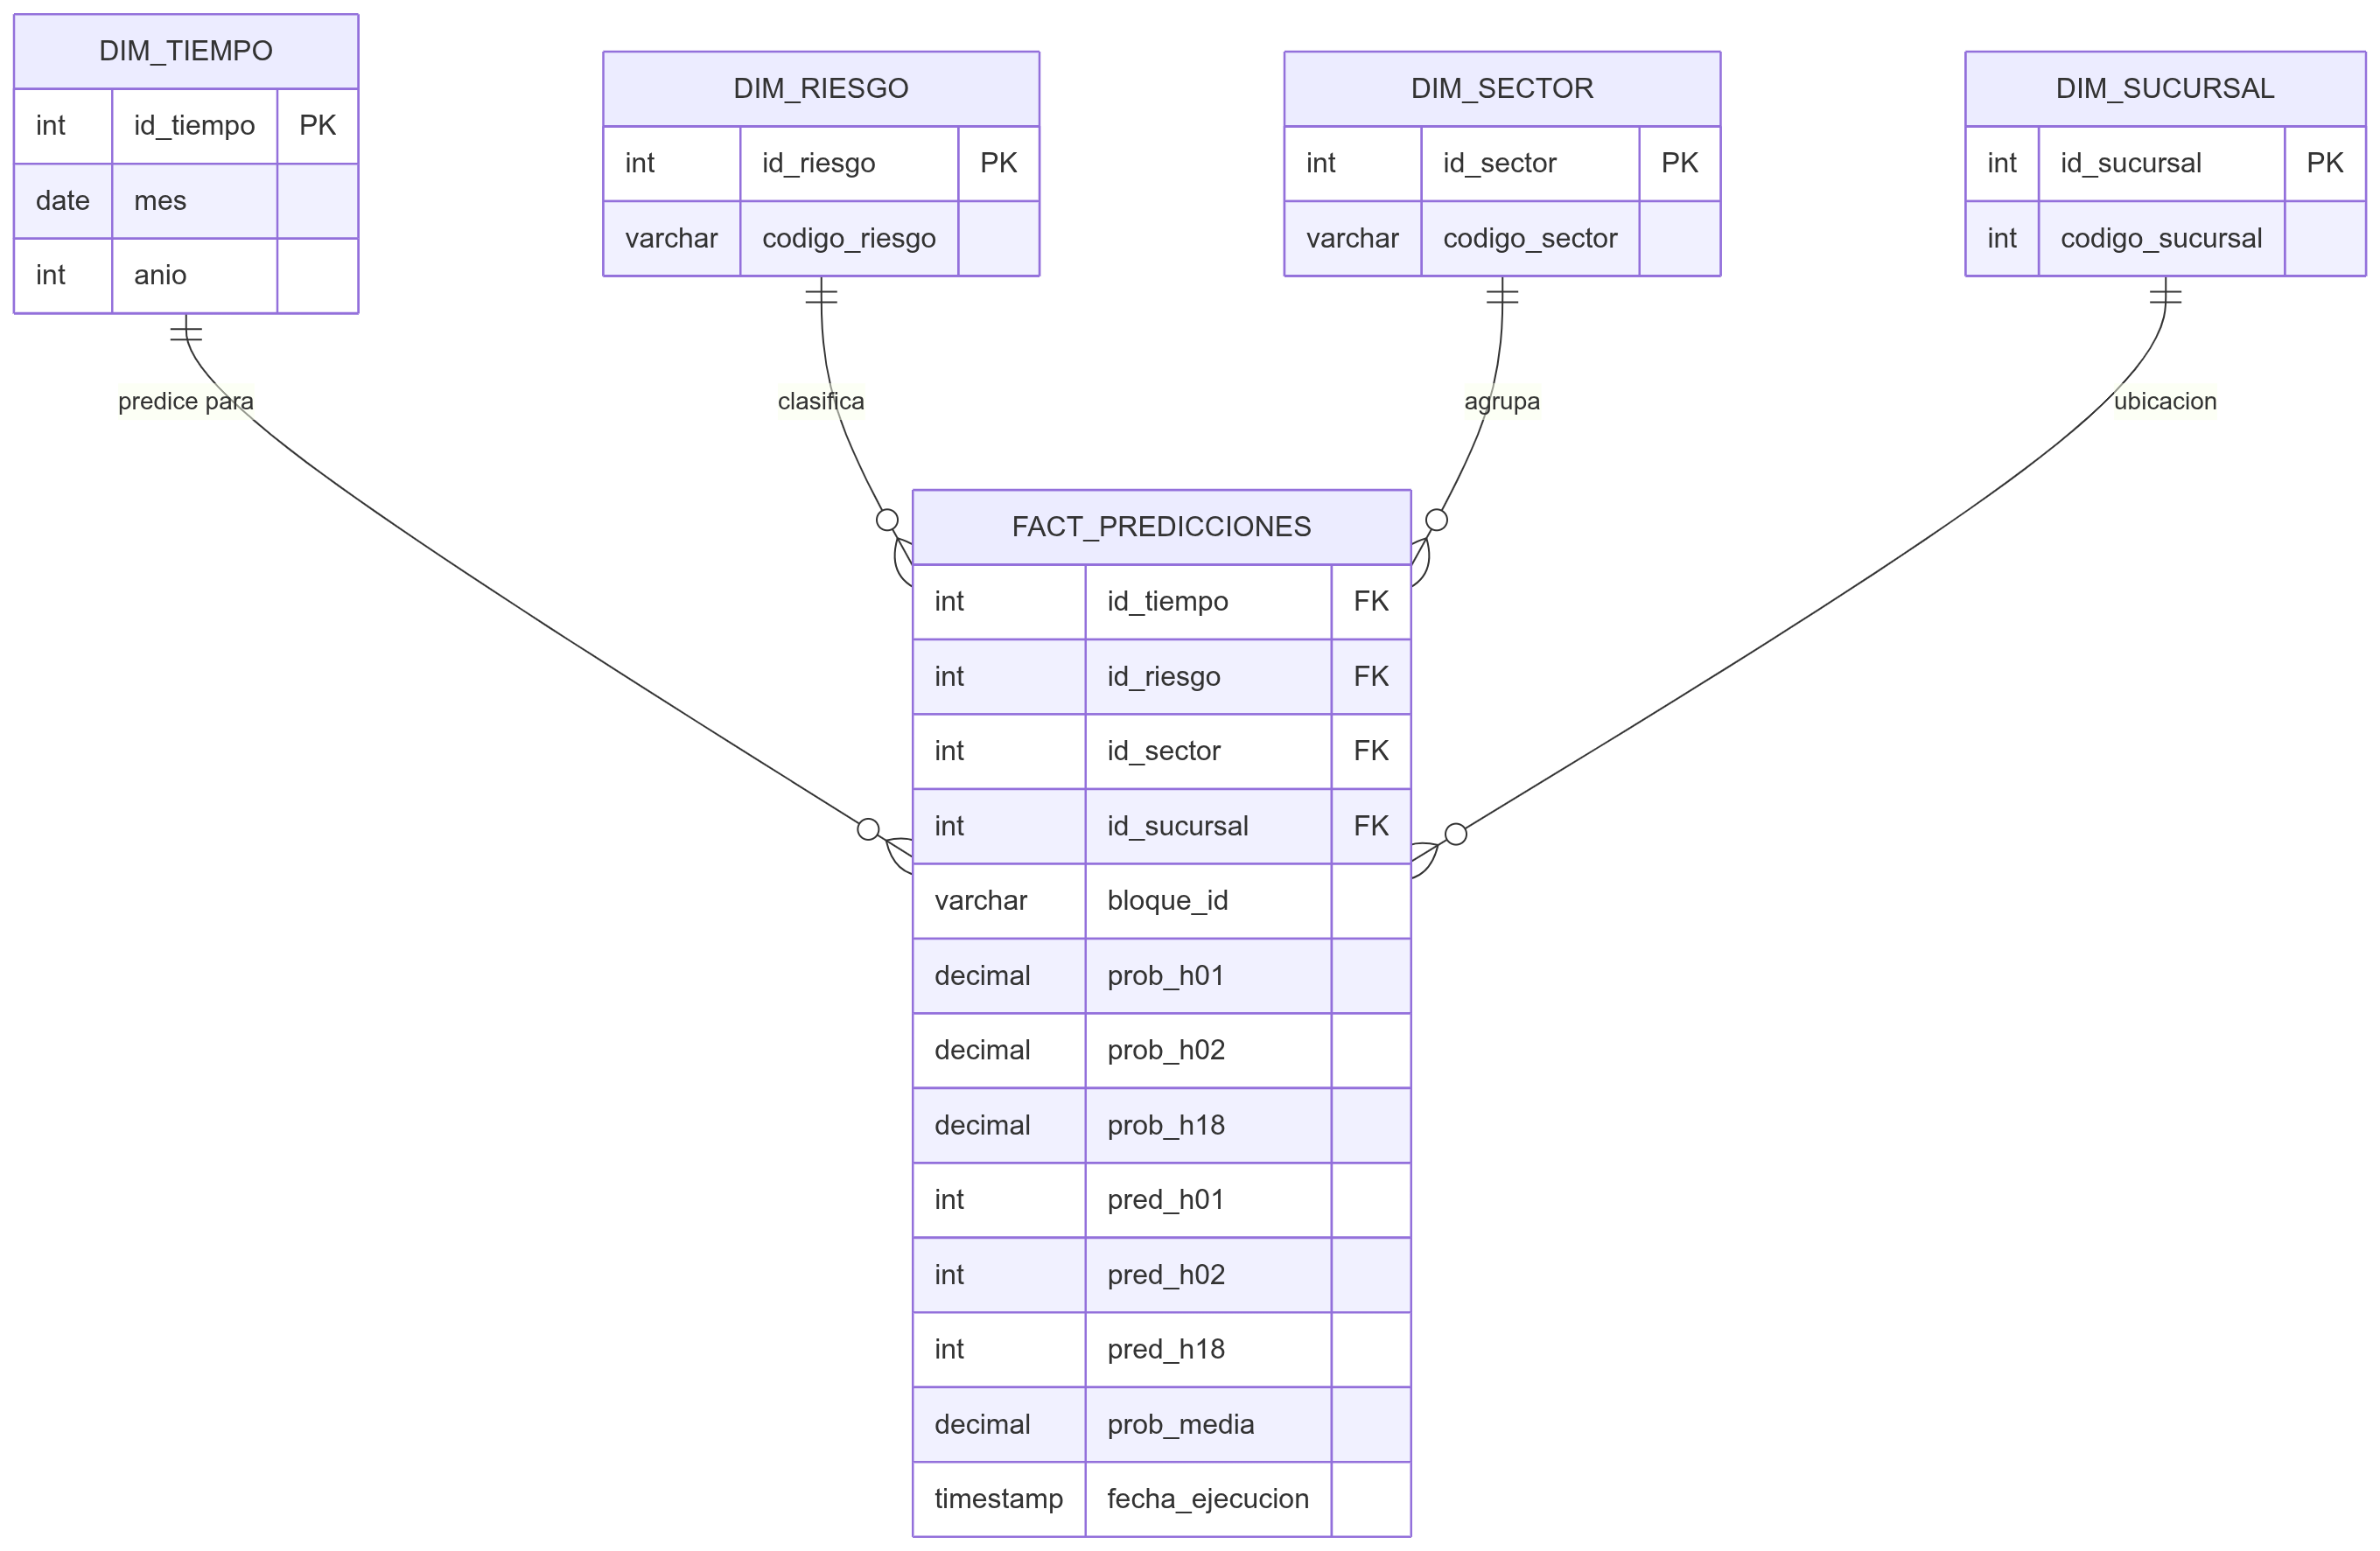
\includegraphics[width=1.0\textwidth]{images/MM-8b Estrella para fact_predicciones.png}
    \caption{Esquema estrella de la tabla \texttt{fact\_predicciones}. Almacena las probabilidades y predicciones binarias para los 18 horizontes temporales, generadas por el modelo seleccionado.}
    \label{fig:appendix_estrella_predicciones}
\end{figure}
\section{Resultados completos de LightGBM por horizonte}

La Tabla~\ref{tab:lgbm_18h} presenta las métricas de los 18 horizontes para el modelo LightGBM bajo el protocolo unificado (entrada de $6 \times 21 = 126$ valores). CNN y MLP no se incluyen por no alcanzar discriminación efectiva en ningún horizonte (AUC-ROC = 0,50 en todos los casos).

\begin{table}[h!]
    \centering
    \small
    \begin{tabular}{|r|r|r|r|r|}
    \hline
    \textbf{Horizonte} & \textbf{Accuracy} & \textbf{Precision} & \textbf{Recall} & \textbf{AUC-ROC} \\
    \hline
        1 mes & 0.8375 & 1.0000 & 0.0008 & 0.8867 \\
    \hline
        2 mes & 0.8797 & 0.6901 & 0.4436 & 0.8873 \\
    \hline
        3 mes & 0.8655 & 0.7508 & 0.2008 & 0.8772 \\
    \hline
        4 mes & 0.8486 & 0.0000 & 0.0000 & 0.8594 \\
    \hline
        5 mes & 0.8545 & 0.0000 & 0.0000 & 0.8501 \\
    \hline
        6 mes & 0.8586 & 0.0000 & 0.0000 & 0.8328 \\
    \hline
        7 mes & 0.8652 & 0.0000 & 0.0000 & 0.8422 \\
    \hline
        8 mes & 0.8674 & 0.4873 & 0.5467 & 0.8319 \\
    \hline
        9 mes & 0.8650 & 0.4632 & 0.5523 & 0.8250 \\
    \hline
        10 mes & 0.8813 & 0.0000 & 0.0000 & 0.8173 \\
    \hline
        11 mes & 0.8666 & 0.4283 & 0.5530 & 0.8219 \\
    \hline
        12 mes & 0.8927 & 0.0000 & 0.0000 & 0.8244 \\
    \hline
        13 mes & 0.8973 & 0.0000 & 0.0000 & 0.8128 \\
    \hline
        14 mes & 0.9017 & 0.0000 & 0.0000 & 0.8138 \\
    \hline
        15 mes & 0.9062 & 0.0000 & 0.0000 & 0.8027 \\
    \hline
        16 mes & 0.9110 & 0.0000 & 0.0000 & 0.8099 \\
    \hline
        17 mes & 0.9164 & 0.0000 & 0.0000 & 0.8054 \\
    \hline
        18 mes & 0.9210 & 0.0000 & 0.0000 & 0.8054 \\
    \hline
        \textbf{Promedio} & \textbf{0.8798} & \textbf{0.2122} & \textbf{0.1276} & \textbf{0.8337} \\
    \hline
    \end{tabular}
    \caption{Métricas completas de LightGBM para los 18 horizontes temporales. La precisión y el recall se calculan con umbral de clasificación 0,5. Solo 5 de los 18 horizontes presentan recall superior a cero, lo que evidencia la dificultad del modelo para identificar la clase minoritaria en horizontes intermedios y largos.}
    \label{tab:lgbm_18h}
\end{table}
